\section{Extension to multiple data sources}\label{sec_same}

Our setup and the results in Section \ref{sec_main} are both for transferring from one data source.
This section extends our setup to transfer learning from multiple data sources.
We focus on a natural setting where all the tasks have the same covariates but different labels.

\paragraph{Data model.} Suppose we have $t$ datasets whose sample sizes are all equal to $n$ and whose feature covariates are all equal to $X \in \real^{n \times p}$. The label vector of the $i$-th task follows a linear model
\begin{align}\label{eq_mtl_data}
    Y^{(i)} = X \beta^{(i)} + \varepsilon^{(i)}, \text{ for } i=1, 2,\cdots, t.
\end{align}
Similar to Section \ref{sec_main}, we use the first $(t-1)$ datasets as sources to predict the $t$-th task.
However, there is a \text{model shift} between the data sources and the task we would like to predict.
We make several standard assumptions on $X$ and each of $\varepsilon^{(i)}$.
First, $X = Z\Sigma^{1/2}$ is a random matrix satisfying Assumption \ref{assm_big1} (same as $X^{(2)}$).
In particular, the sample size $n$ is greater than the dimension $p$.
Second, every $\varepsilon^{(i)} \in \real^{n}$ is a random vector with i.i.d entries of mean zero, variance $\sigma^2$, and bounded moments up to any order (cf. equation \eqref{eq_highmoments}).
Finally, $\beta^{(i)} \in \real^{p}$ is a fixed vector independent from any other $\beta^{(j)}$ for $j \neq i$, the matrix $X$, and $\varepsilon^{(j)}$ for any $j=1,\dots,t$.

\paragraph{Estimator.} We combine multiple data sources by extending the two-layer linear neural network from equation \eqref{eq_hps} as follows:
\begin{align}
	f(A, B) = \sum_{j=1}^t \bignorm{X B A_j - Y^{(j)}}^2, \label{eq_mtl_same_cov}
\end{align}
where $A = [A_1, A_2, \dots, A_t] \in \real^{r \times t}$ denotes the output layer and $B \in \real^{p \times r}$ denotes the (shared) feature layer.
We set the width of the feature layer $r$ less than the number of tasks $t$.
Otherwise, when $r \ge t$, the global minimum of $f(A, B)$ reduces to single-task learning, similar to Proposition \ref{prop_large_r} (details omitted).

Let $(\hat A, \hat B)$ denote a global minimizer of $f(A, B)$.
We define the HPS estimator for task $i$ as $\hat \beta_i^{\MTL} := \hat B \hat A_i$, where $\hat A_i$ denotes the $i$-th column of $\hat A$.
We evaluate the performance of $\hat{\beta}_i^{\MTL}$ according to its excess risk:
\be\label{ith_loss}
    L_i(\hat{\beta}_i^{\MTL}) = \bignorm{\Sigma^{1/2} \left(\hat{\beta}^{\MTL}_i - \beta^{(i)}\right)}^2.
\ee

\paragraph{Result.} We show that in the multi-task setting, hard parameter sharing finds the ``best'' rank-$r$ approximation to all tasks.
To formally describe our result, we introduce several notations.
Let $B^\star \define [{\beta}^{(1)},{\beta}^{(2)},\dots,{\beta}^{(t)}] \in \real^{p\times t}$ be the concatenated model vectors of all tasks.
Let $A^{\star} {A^{\star}}^{\top}$ be the best approximation of ${B^{\star}}^\top\Sigma B^{\star}$ in the set of rank-$r$ subspaces:
\begin{align}\label{eq_A_star}
	A^{\star} \define \argmax{U\in\real^{t\times r} : U^{\top} U = \id_{r\times r}} \inner{U U^{\top}} {{B^{\star}}^{\top} \Sigma B^{\star}},
\end{align}
where $\langle \cdot ,\cdot \rangle $ denotes the Frobenius inner product between two matrices.
Let $a_i^{\star}\in\real^r$ be the $i$-th column vector of $A^{\star}{A^{\star}}^{\top}$.
We show a precise estimate of $L_i(\hat{\beta}_i^{\MTL})$ based on $a_i^{\star}$ as follows.

\begin{theorem}[Excess risk of HPS for multiple tasks under model shift]\label{thm_many_tasks}
Suppose the multi-task setting according to equation \eqref{eq_mtl_data} holds.
Let $r < t$ be a positive integer.
Suppose the $r$-th largest eigenvalue of ${B^\star}^\top \Sigma B^\star$ is strictly larger than its $(r+1)$-th largest eigenvalue. 
Let $c>0$ be an arbitrarily (small) constant.
The following estimate of $L_i(\hat{\beta}_i^{\MTL})$ holds w.h.p., for any $i = 1,\dots,t$:
\begin{align}
	\bigabs{L_i(\hat{\beta}_i^{\MTL}) - L_i(B^{\star}a_i^{\star}) -\frac{p\sigma^2}{n-p} \cdot \norm{a_i^{\star}}^2} 
	\le  \sqrt{\norm{{B^\star}^\top\Sigma B^\star}_{2} \cdot n^{-\frac 1 2+ \frac 2{\varphi} + c}  + \sigma^2 n^{-\frac 1 2 + c}} \cdot \frac{\norm{{B^\star}^\top\Sigma B^\star}_{2}+  \sigma^2}{\lambda_r - \lambda_{r+1}}. \label{Li_multi1}
\end{align}
	%where $\lambda_r({B^\star}^\top\Sigma B^\star)$ and $\lambda_{r+1}({B^\star}^\top\Sigma B^\star)$ are respectively be the $r$-th and $(r+1)$-th largest eigenvalue of ${B^\star}^\top\Sigma B^\star$.
%	where $C_1: = \frac{\bignormFro{\Sigma^{1/2} B^{\star}}^2 + \sigma^2 t}{\lambda_r ({B^\star}^\top \Sigma B^\star)- \lambda_{r+1}({B^\star}^\top \Sigma B^\star)}$. %and $C_2 :=  C_1\cdot \norm{\Sigma^{1/2} B^{\star}}$.
%Finally, we have a better bound for the averaged prediction loss:  with high probability,
%\begin{align}
%&\left|\frac{1}{t}\sum_{i=1}^t L_i(\hat{\beta}_i^{\MTL}) - \frac1t\bignorm{\Sigma^{1/2} B^{\star} (A^\star {A^\star}^{\top} - \id_{t\times t})}_F^2 - \frac{p \sigma^2}{n-p}\cdot \frac{r}{t}  \right| \nonumber \\
% &\le n^{-1/2+2/\varphi+c}  \norm{{B^\star}^\top\Sigma B^\star}+ n^{-1/2+c}   \sigma^2 .\label{Li_multi2}
%\end{align}
\end{theorem}


Recall that $\varphi > 4$ according to Assumption \ref{assm_big1}, thus, $\frac {2}{\varphi} \le \frac 1 2$ and $n^{-\frac 1 2 + \frac 2 {\varphi} + c}$ vanishes to zero for a small enough constant $c$.
Thus, $L_i(B^{\star} a_i^{\star}) + \frac{p\sigma^2}{n - p} \norm{a_i^{\star}}^2$ is the limit of $L_i(\hat{\beta}_i^{\MTL})$ as $p$ approaches infinity---$L_i(B^{\star} a_i^{\star})$ is the limiting bias of $\hat{\beta}_i^{\MTL}$ and $\frac{p \sigma^2}{n - p} \bignorm{a_i^{\star}}^2$ is its limiting variance.
The proof of Theorem \ref{thm_many_tasks}, which characterizes the global minimum of problem \eqref{eq_mtl_same_cov} through a connection to PCA, can be found in Section \ref{app_proof_error_same_cov}.
%We also point out that equation \eqref{Li_multi1} similarly applies to any other task $t' \neq t$.
%The bound \eqref{minimizer_beta} verifies our intuition that hard parameter sharing approximates the matrix ${B^{\star}}^\top\Sigma B^{\star}$ through a best rank-$r$ subspace. The estimate \eqref{Li_multi1}
% gives the exact asymptotic limit of $L_i(\hat{\beta}_i^{\MTL}(\hat a))$, which shows that the prediction loss of $\hat{\beta}_i^{\MTL}$ decomposes into a bias term $L_i(B^{\star} a_i^{\star})$ that measures the prediction loss of $B^{\star} a_i^{\star}$, plus a variance term that scales with $\norm{a_i^{\star}}^2$. Since $\norm{a_i^{\star}}^2\le 1$, compared with the single-task predication loss \eqref{L_STL_simple01}, the variance term always decreases for the multi-task HPS estimator. On the other hand, the bias term always increases (because the bias in single-task linear regression is zero). Hence as in the transfer learning setting, whether the HPS estimator is better than the OLS estimator depends on an intricate  {bias-variance tradeoff}.
%{\cor One direct implication of our result is that compared to STL, the variance always decreases, since STL's variance is equal to $\sigma^2 \tr[\Sigma (X^{\top} X)^{-1}]$.
%On the other hand, the bias always increases.}
%We can observe a similar {bias-variance tradeoff} for the averaged predication loss in \eqref{Li_multi2} using the fact that $r<t$. Note that the estimate \eqref{Li_multi2} can be applied even when the best rank-$r$ subspace approximation of ${B^{\star}}^\top\Sigma B^{\star}$ is not unique. For all the estimates in Theorem \ref{thm_many_tasks}, we believe that their convergence rates are asymptotically tight when $n$ goes to infinity.
%	For the optimization objective  in \eqref{eq_mtl_same_cov}, using the local optimality condition over $B$, that is, $\frac{\partial f}{\partial B} = 0$, we obtain $\hat{B}$ as a function of $A$:
%	\begin{align}
%		\hat{B}(A) %&\define (X^{\top}X)^{-1} X^{\top} \bigbrace{\sum_{j=1}^t Y^{(j)} A_j^{\top}} (A  A^{\top})^{+} \nonumber \\
%		&= (X^{\top} X)^{-1} X^{\top} Y A^{\top} (AA^{\top})^{+}, \label{eq_Bhat}
%	\end{align}
%	where $Y := [Y^{(1)}, Y^{(2)}, \dots, Y^{(t)}]$ and $(AA^{\top})^{+}$ denotes the pseudoinverse of $AA^{\top}$.
	%Here we have used that $X^{\top}X$ is invertible since $n > \rho \cdot p$ and $\rho > 1$ (cf. Fact \ref{fact_minv}).
	%\FY{Is $\dag$ a standard notation? It is a bad notation at least for me because $\dag$ is more often used as Hermitian conjugate. Wiki page uses $(AA^{\top})^{+}$ for pseudo-inverse.}
%	Plugging $\hat{B}(A)$ into equation \eqref{eq_mtl_same_cov}, we obtain the following objective that only depends on $A$ (in matrix notation):
%	\begin{align}\label{eq_mtl_output_layer}
%		g(A) = \bignormFro{X (X^{\top}X)^{-1}X^{\top} Y A^{\top} (AA^{\top})^{+} A - Y}^2.
%	\end{align}


%Moreover, by setting $t=2$ in Theorem \ref{thm_many_tasks}, we can obtain the prediction loss for the HPS estimator for the transfer learning setting where the two tasks have the same covariates  $X^{(1)}=X^{(2)}$. For the reader's convenience, we give the precise statement in Corollary \ref{thm_two_tasks}.
%Theorem \ref{thm_many_tasks} implies Theorem \ref{thm_two_tasks} as a special case with $t=2$ and $r=1$.
%In this section, we consider the setting where the two tasks have the same covariates  $X^{(1)}=X^{(2)}$.
%We define $A^\star \in \R^{2}$ as the normalized eigenvector corresponding to the larger eigenvalue of the $2\times 2$ matrix
%$ {B^\star}^\top \Sigma  B^\star,$ where recall that $B^\star \define [{\beta}^{(1)},{\beta}^{(2)}] \in \real^{p\times 2}$ by definition.
% is the matrix formed by the linear model parameters of the two tasks.
%Without loss of generality, we assume that the two eigenvalues of ${B^\star}^\top \Sigma B^\star$ are not degenerate, so that $A^\star$ is uniquely defined. %Otherwise, Theorem \ref{thm_two_tasks} will give a null result.
%In the following corollary, the estimate \eqref{minimizer_beta1} shows that the minimizer $\hat a$ is approximately equal to $A^\star(1)/A^\star(2)$, while \eqref{Li_multi0} gives the exact asymptotic limit of $L_2(\hat{\beta}_2^{\MTL}(\hat a)) $, together with an explicit convergence rate that we believe to be sharp.

%\begin{corollary}\label{thm_two_tasks}
%Under Assumption \ref{assm_big1}, suppose that $X^{(1)}=X^{(2)}$ and $n_1=n_2\equiv n$. Let $c>0$ be an arbitrary (small) constant. Then we have that with high probability,
%\be\label{minimizer_beta1}
%\left\| u_{\hat a}u_{\hat a}^\top - A^\star {A^\star}^\top\right\|_F  \le  \left[\frac{ n^{-1/2+2/\varphi+c}  \|{B^{\star}}^{\top}\Sigma B^{\star}\|  + n^{-1/2+c} \sigma^2 }{\lambda_1 - \lambda_{2} } \right]^{1/2},
%\ee
%where $u_{\hat a}$ is the unit vector defined as
%$ u_{\hat a}:= \frac1{\hat a^2 +1} \begin{pmatrix} {\hat a}\\ %1\end{pmatrix},$ and $\lambda_1 $ and $\lambda_{2}$ are respectively the larger and smaller eigenvalues of ${B^\star}^\top\Sigma B^\star$.
%for task 2,  % over the randomness of the input,
%Moreover, the prediction loss of the HPS estimator satisfies that with high probability,
%	\begin{align}
%		& \bigabs{L_2(\hat{\beta}_2^{\MTL}(\hat a)) - \left\|(\Sigma^{(2)})^{1/2} \left(A^\star(2) \cdot B^{\star}A^{\star}  - \beta^{(2)}\right)\right\|^2  - |A^\star(2)|^2  \frac{p\sigma^2}{n-p} } \nonumber\\
%		& \le  \left[  \frac{  n^{-1/2+2/\varphi+c} \|{B^{\star}}^{\top}\Sigma B^{\star}\|+n^{-1/2+c} \sigma^2} {\lambda_1  - \lambda_2 }\right]^{1/2}   \left(\norm{\Sigma^{1/2} B^{\star}}^2+  \sigma^2\right), \label{Li_multi0}
		%\le n^{-\frac{c_{\varphi}}2} \cdot \frac{\bigbrace{ \norm{\Sigma^{1/2} B^{\star}}^2+  \sigma^2} \cdot (\bignormFro{\Sigma^{1/2} B^{\star}}^2 + \sigma^2 t)} {\lambda_r ({B^\star}^\top \Sigma B^\star)- \lambda_{r+1}({B^\star}^\top \Sigma B^\star)},
%	\end{align}
%	 where $A^\star(2)$ denotes the second entry of $A^\star$.
%	 \end{corollary}

\begin{figure}[!t]
	\begin{subfigure}[b]{0.5\textwidth}
		\centering
		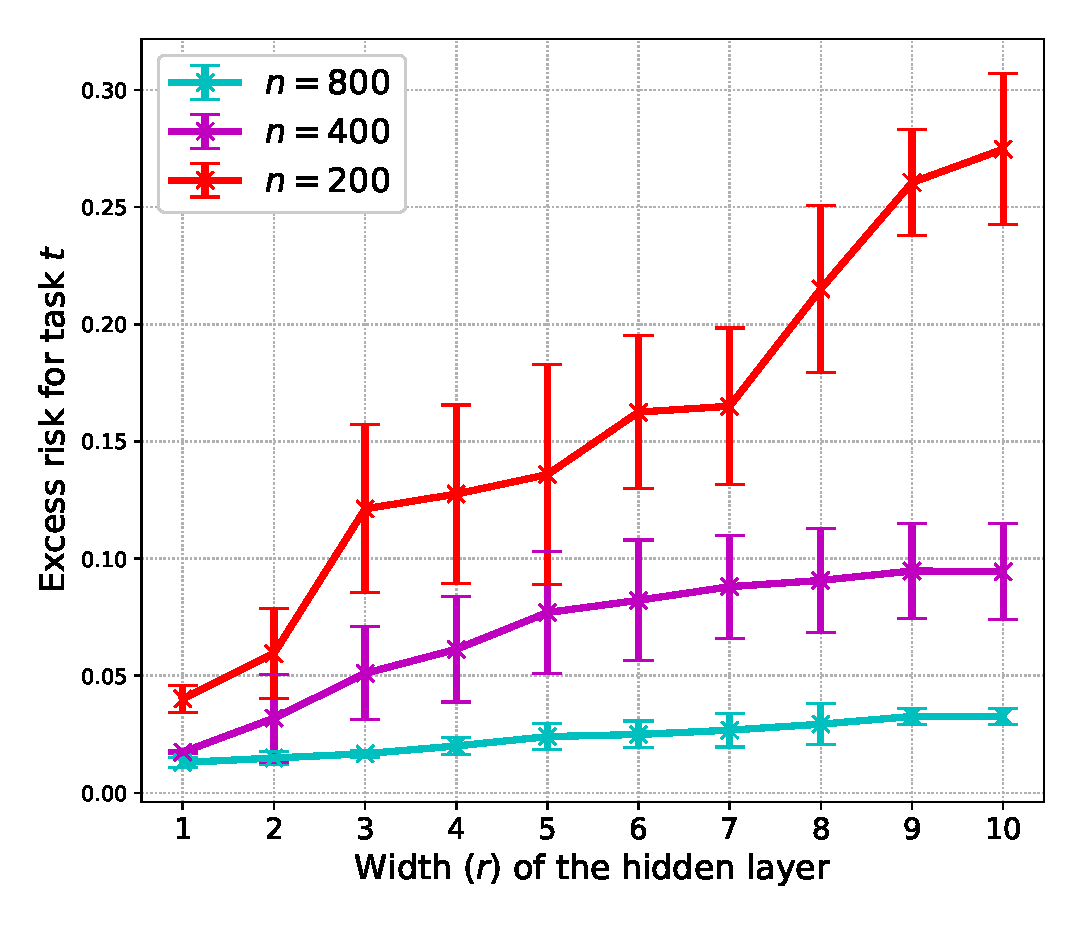
\includegraphics[width=0.8\textwidth]{figures/multitask_width.eps}
		\caption{Varying width}
		\label{fig_sec4_width}
	\end{subfigure}
	\begin{subfigure}[b]{0.5\textwidth}
		\centering
		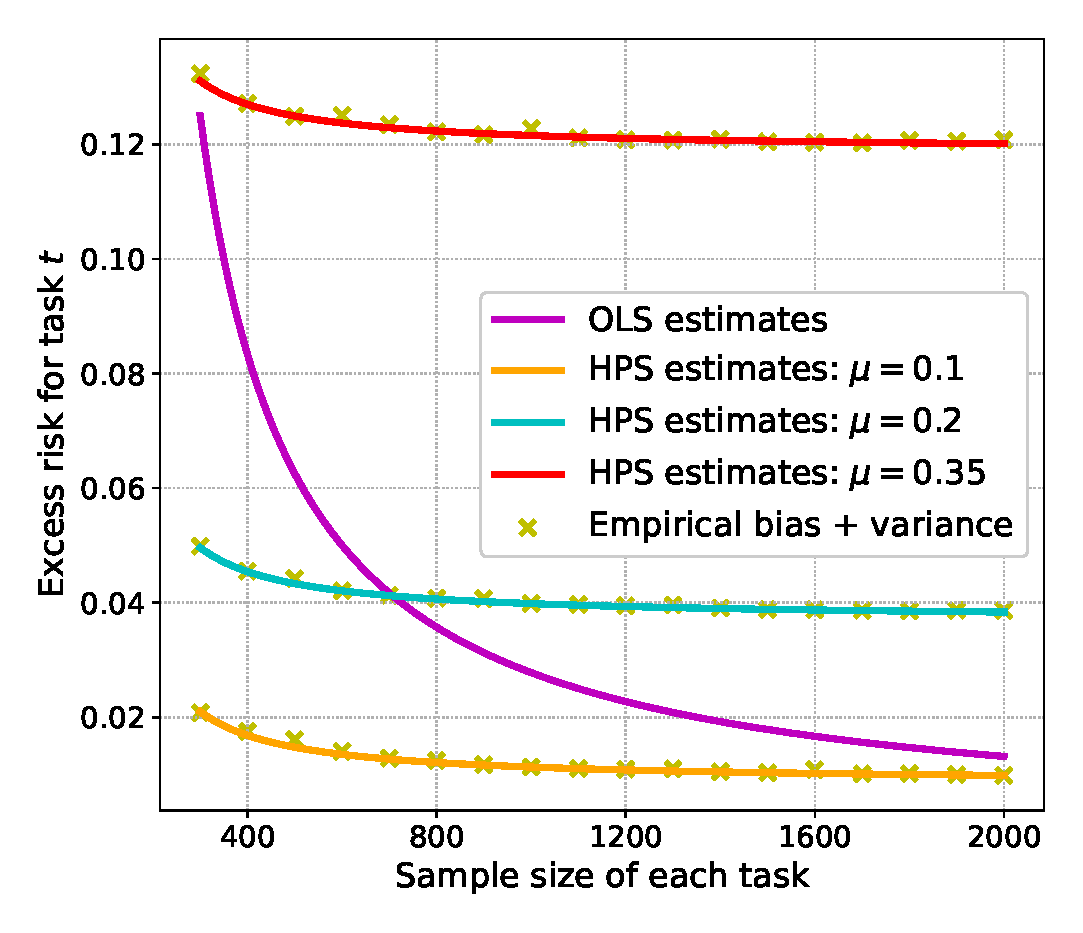
\includegraphics[width=0.8\textwidth]{figures/multitask_transfer.eps}
		\caption{Varying sample size and model shift parameter}
		\label{fig_sec4_transfer}
	\end{subfigure}
	\caption{We illustrate the performance of HPS in the random-effect model with $p = 100, t = 10, \sigma = 1/2$.
	Figure \ref{fig_sec4_width} shows that from $1$ to $t = 10$, setting width $r = 1$ gives the lowest excess risk for task $t$.
	The result is averaged over three random seeds.
	This simulation uses $\mu = 0.05$.
	Figure \ref{fig_sec4_transfer} fixes $r = 1$ while varying $\mu$ and $n$. We observe that depending on $\mu$ and $n$, HPS may provide a positive transfer or a negative transfer to task $t$ (similar to Figure \ref{fig_sec3_model_shift}). The precise condition for deciding which one is provided in Claim \ref{claim_re_multi}.}
	\label{fig_sec4}
\end{figure}


\paragraph{Illustrative examples.}
We give an example of our estimate in the random-effect model.
In this setting, the model vector of every task is the sum of a shared vector $\beta_0$ plus a task-specific component $\wt \beta^{(i)}$:
\begin{align}
    \beta^{(i)} = \beta_0 + \wt \beta^{(i)}, \text{ for every } i=1,2,\cdots, t, \label{eq_re_mt}
\end{align}
where every entry of $\wt \beta^{(i)}$ is drawn i.i.d. from a Gaussian distribution with zero mean and ${\mu^2}/p$ variance.
Thus, $\mu$ is a parameter for modeling the difference between different tasks.
We study two fundamental questions in this setting.
First, what should the width ($r$) of the feature layer $B$ be?
Second, when does HPS transfer positively to a particular task, depending the sample size $n$ and the (model shift) parameter $\mu$?
Since all tasks are symmetric in this setting, we analyze the average (limiting) risk
\[ g_r(n, \mu) = \frac {1}{t} \sum_{i=1}^t \big(L_i(B^{\star} a_i^{\star}) + \frac{p \sigma^2}{n - p} \cdot \norm{a_i^{\star}}^2\big). \]
We address both questions by characterizing $g_r(n, \mu)$, which accurately approximates $\frac{1}{t} \sum_{i=1}^t L_i(\hat{\beta}_i^{\MTL})$ according to Theorem \ref{thm_many_tasks}.
Recall from Lemma \ref{lem_hat_v} that the excess risk of the OLS estimator satisfies that $L_i(\hat{\beta}_i^{\STL}) = \frac{\sigma^2 p}{n - p} + o_p(1)$, in which $o_p(1)$ vanishes to zero as $p$ approaches infinity.
We compare $g_r(n, \mu)$ with the OLS estimate in the following claim.
\begin{claim}[Choosing $r$ for HPS in the random-effect model]\label{claim_re_multi}
    Suppose the multi-task setting with random-effect linear models under equation \eqref{eq_mtl_data} and \eqref{eq_re_mt} holds.
    Let $\epsilon = o_p(\norm{\beta_0}^2 + \mu^2)$ be a small error term that decreases to zero as $p$ goes to infinity.
    Let $r \in [1, r]$.
    W.h.p. over the randomness of $B^{\star}$, the following holds:
    \begin{enumerate}
        \item[i)] If $\mu^2 \ge \frac{\sigma^2 p^2}{(n - p) \tr[\Sigma]}$, then $g_r(n, \mu) \ge \frac{\sigma^2 p}{n - p} + \epsilon$, for any $1\le r < t$.
    	\item[i)] If $\mu^2 < \frac{\sigma^2 p^2}{(n - p)\tr[\Sigma]} - \frac{t p}{\bigtr{\Sigma}} \epsilon$, then $g_r(n, \mu)$ is minimized when $r=1$.
    	Additionally, $g_1(n, \mu) \le \frac{\sigma^2 p}{n - p} + \epsilon$.
    \end{enumerate}
\end{claim}
%For our discussion below, we assume that $\kappa^2 \sim d^2 \sim \sigma^2$ and $n\sim p$. %and $d^2=\OO(\kappa^2)$.
%The more precise conditions on the relations between $d^2$, $\sigma^2$ and $\kappa^2$ are given in  \eqref{choiceofpara}.
%We assume that all the random variables have finite moments up to any order as in equation \eqref{assmAhigh2}.
\begin{proof}
    We first simplify the expression of $g_r(n, \mu)$ using its definition
    \begin{align*}
        g_r(n, \mu) &= \frac 1 t \sum_{i=1}^t \big(L_i(B^{\star} a_i^{\star}) + \frac{p\sigma^2}{n - p} \cdot \norm{a_i^{\star}}^2\big) \\
        &= \Big(\frac 1 t \sum_{i=1}^t \bignorm{\Sigma^{1/2} (B^{\star} a_i^{\star} - \beta^{(i)})}^2 \Big)
        + \Big(\frac 1 t \sum_{i=1}^t \frac{p\sigma^2}{n - p} \cdot \norm{a_i^{\star}}^2 \Big) \\
        &= \frac 1 t \bignormFro{\Sigma^{1/2} (B^{\star} A^{\star} - B^{\star})}^2 + \frac{r}{t} \cdot \frac{p\sigma^2}{n - p}.
    \end{align*}
    In the last step, we use the matrix notation to write the sum for the first part.
    We use the fact that $\sum_{i=1}^t \norm{a_i^{\star}}^2 = r$ because $A^{\star} = [a_1^{\star}, \dots, a_t^{\star}]$ satisfies that ${A^{\star}}^{\top} A^{\star} = \id_{p\times p}$ following its definition in equation \eqref{eq_A_star}.
    Using this condition on $A^{\star}$, we further get that
    \begin{align*}
        \bignormFro{\Sigma^{1/2}(B^{\star} A^{\star} - B^{\star})}^2
        = \bigtr{{B^{\star}}^{\top} \Sigma B^{\star} (\id_{p \times p} - A^{\star}{A^{\star}}^{\top})},
    \end{align*}
    which is precisely equal to the smallest $(t - r)$ eigenvalues of ${B^{\star}}^{\top}\Sigma B^{\star}$.
    Using the concentration of Gaussian random vectors in Lemma \ref{largedeviation}, w.h.p. the $(i, j)$-th entry of ${B^{\star}}^{\top} \Sigma B^{\star}$ is equal to
    \begin{align}\label{betaSbeta}
    	{\beta^{(i)}}^{\top}\Sigma  {\beta^{(j)}} =\beta_0^\top \Sigma \beta_0 + \delta_{i,j} \frac{\mu^2 }{p}\bigtr{\Sigma} + \OO\left(p^{-1/2+c}\|\beta_0\|^2+ p^{-1/2+c} \mu^2\right)
    \end{align}
    for any constant $c>0$, where $\delta_{i,j} = 1$ if and only if $i = j$.
    Thus, ${B^{\star}}^{\top} \Sigma B^{\star}$ is equal to a rank-$1$ matrix with (spectral) norm $t\cdot \beta_0^{\top} \Sigma \beta_0$ plus Gaussian perturbation.
    Using the concentration result of Lemma \ref{largedeviation} \todo{check}, we have that
    \begin{align*}
        \lambda_1 &= \Big(1+\OO(p^{-1/2+c})\Big)\cdot\left(t\cdot \beta_0^\top \Sigma \beta_0  + \frac{\mu^2}{ p}\bigtr{\Sigma}\right) , \text{ and } \\
        \lambda_i &= \Big(1+\OO(p^{-1/2+c})\Big)\cdot \frac{\mu^2}{ p}\bigtr{\Sigma}, \text{ for } i=2,\cdots, t.
    \end{align*}
    Thus, w.h.p. the sum of smallest $(t - r)$ eigenvalues of ${B^{\star}}^{\top}\Sigma  B^{\star}$ is equal to
    $(1+\OO(p^{-1/2+c}))\cdot(t-r)\frac{\mu^2 \bigtr{\Sigma}}{p}$.
    Let $\epsilon = o_p(1)$ denote the error term.
    %To see this, recall that $r$ is one and $A^{\star} {A^{\star}}^{\top}$ is the best rank-$1$ approximation of ${B^{\star}}^{\top}\Sigma B^{\star} = {B^{\star}}^{\top} B^{\star}$.
    %Hence, the above expression is equal to the sum of ${B^{\star}}^{\top} {B^{\star}}$'s bottom $t-1$ singular values.
    %In the random-effect model described above, we further assume that $\Sigma$ is isotropic as an example.
    %We show that when the rank $r$ is one, the average prediction loss of hard parameter sharing is as follows
    We conclude that w.h.p.,
    \begin{align}
        g_r(n, \mu) - \frac{\sigma^2 p}{n - p} &= \bigbrace{1 - \frac{r}{t}} \frac{\mu^2}{p}\bigtr{\Sigma} + \frac{r}{t} \cdot \frac{p\sigma^2 }{n - p} + \epsilon - \frac{\sigma^2 p}{n - p} \nonumber \\
        &= \Big(1 - \frac r t\Big) \cdot \Big(\frac{\mu^2\bigtr{\Sigma}}{p} - \frac{p\sigma^2}{n - p}\Big) + \epsilon. \label{eq_re_final}
    \end{align}
    Now we are ready to finish the proof.
    For claim i), if $\mu^2 \ge \frac{\sigma^2 p^2}{(n - p) \bigtr{\Sigma}}$, the coefficient of $(1 - \frac r t)$ in equation \eqref{eq_re_final} is non-negative, and claim i) follows.
    For claim ii), if $\mu^2 < \frac{\sigma^2 p^2}{(n - p)\bigtr{\Sigma}} - \frac{p t}{\bigtr{\Sigma}}\epsilon$, the coefficient of $(1 - \frac r t)$ in equation \eqref{eq_re_final} is negative.
    Furthermore, equation \eqref{eq_re_final} is minimized when $r = 1$, and claim ii) follows since the RHS of equation \eqref{eq_re_final} is at most $\epsilon$.
\end{proof}


Figure \ref{fig_sec4} validates Claim \ref{claim_re_multi}.
First, we see that the empirical excess risk (measured on a particular task) is indeed smallest when the width $r$ is equal to $1$.
Second, we see that HPS provides a positive transfer (to a particular task) depending on the sample size $n$ and the model shift parameter $\mu$.
The results match with the condition (on $\mu$) suggested by our estimates.













%\FY{add simulations to check our results; discuss motivations and possible applications}
\iffalse
In this paper, we consider a natural extension of the estimator $\hat \beta^{\rm{TL}} $, that is, the \emph{hard parameter sharing} (HPS) estimator, which has been a standard type of estimator in multi-task learning \FY{citations}. More precisely, we study the following HPS architecture: a shared feature representation layer $B\in\real^{p}$ for all datasets and a separate output layer $A_i \in \real$ for every dataset $i$. Then we study the following minimization problem:
\begin{align}\label{eq_tsl}
			f(A, B) = \norm{X^{(1)} B A_1 - Y^{(1)}}^2 + \norm{X^{(2)} B A_2 - Y^{(2)}}^2,
\end{align}
where we abbreviate $A = [A_1, A_2]$. Let $(\hat{A}, \hat{B})$ be the minimizer of $f(A, B)$. We define the hard parameter sharing (HPS) estimator for task $i$ as
\be\label{def_HPS}\hat{\beta}_i^{\MTL} = \hat{B} \hat{A}_i,\quad i=1,2.\ee
Note that $\hat \beta^{\rm{TL}}$ is a special case of $\hat{\beta}_i^{\MTL}$ by setting $A_1=A_2=1$.

For the optimization objective $f(A, B)$ in \eqref{eq_tsl}, using the local optimality condition $\frac{\partial f}{\partial B} = 0$, we can solve that
	\begin{align}
		\hat{B} = A_2^{-1} \hat \Sigma(a)^{-1} \left[a (X^{(1))})^{\top}Y^{(1)} +  (X^{(2)})^{\top}Y^{(2)}\right], \label{eq_Bhat_2task} %\\
		%&= (B^\star A ^{\top}) (A A^{\top})^{-1} + (X^{\top}X)^{-1}X^{\top}   \bigbrace{\sum_{j=1}^t \varepsilon_i A_i^{\top}} (A  A^{\top})^{-1}.
	\end{align}
where we denote $a:=A_1/A_2$ and $\hat \Sigma(a):= a^2 (X^{(1)})^\top X^{(1)}  + (X^{(2)})^\top X^{(2)}$.
Applying $\hat B$ to equation \eqref{eq_tsl}, we obtain an objective that only depends on $a $ as follows %\HZ{$A$ has been used to denote the output layers. Could you replace $A$ with another symbol (say $x$)?}
 \begin{align}
		 g(a) \define & \left\| X^{(1)} \hat\Sigma(a)^{-1} (X^{(2)})^\top X^{(2)} (a\beta^{(2)}-\beta^{(1)}) \right. \nonumber\\
			& \left. + \left(a^2 X^{(1)}\hat \Sigma(a)^{-1} (X^{(1)})^\top-\id_{n_1\times n_1}\right)\epsilon^{(1)}+ a X^{(1)}\hat \Sigma(a)^{-1} (X^{(2)})^\top \epsilon^{(2)} \right\|^2 \nonumber\\
		   +& \left\| X^{(2)} \hat \Sigma(a)^{-1} (X^{(1)})^\top X^{(1)} (a\beta^{(1)}-a^2\beta^{(2)}) \right. \nonumber\\
		  &\left.+ \left(X^{(2)}\hat\Sigma(a)^{-1} (X^{(2)})^\top-\id_{n_2\times n_2}\right)\epsilon^{(2)} + a X^{(2)}\hat \Sigma(a)^{-1} (X^{(1)})^\top \epsilon^{(1)} \right\|^2. \label{eq_mtl_A12}
	\end{align}
Let $\hat a$ be the minimizer of $g(a)$. Throughout this paper, we regard $Y^{(1)}$ as the source data, and $Y^{(2)}$ as the target data.  Then the HPS estimator \eqref{def_HPS} for the target task 2 is
\be\label{HPS_est}
\hat{\beta}_2^{\MTL} (\hat a) = \hat \Sigma(\hat a)^{-1}  \left[\hat a (X^{(1))})^{\top}Y^{(1)} +  (X^{(2)})^{\top}Y^{(2)}\right].
\ee
\fi
